\begin{solution}[label=ques:3]
  \begin{question}
    Give two different decompositions of the 1-qubit mixed state $$\rho = \begin{bmatrix}\cos^2(\pi/8) & 0\\ 0 & \sin^2(\pi/8)\end{bmatrix}$$ as a mixture of two pure states. Show your work. What do these decompositions correspond to physically?
Draw a 2D-sketch of the Bloch sphere to aid your explanation.
  \end{question}
  \tcblower{}
  \begin{proof}[Solution]
    One trivial decomposition for the given state $\rho$ is $\cos^2\pi/8$ probability of having the $\ket{0}$ state and $\sin^2\pi/8$ probability of measuring the $\ket{1}$ state.\par
    Now, for obtaining a second possible decomposition, we compute the coefficients of $\rho$ in the generalised representation of any state in the Bloch sphere. We have
    \begin{equation}
      \begin{split}
        &\rho = \frac{1}{2}\left(\bfI + x\bfX + y\bfY + z\bfZ\right)\\
        \implies &\cos^\pi/8 = 1 + z, \sin^2\pi/8 = 1 - z, x + iy = 0, x - iy = 0\\
        \implies &z = 2\cos^2\pi/8 - 1 = \cos\pi/4 = \frac{1}{\sqrt{2}}, x = y = 0
      \end{split}
      \label{eq:blochdecomp}
    \end{equation}
    Therefore, the state $\rho$ is on the $Z$ axis with the $z$ coordinate of $\frac{1}{\sqrt{2}}$. Now, let us try to decompose the state with one state as the $\ket{+}$ state (this has coordinates $(1, 0, 0)$). Now, let us assume that the other state $\ket{\psi}$ will have coordinates $(x, y, z)$. We can write $\rho$ in terms of density matrices given by $\ket{+}$ and $\ket{\psi}$ as
    \begin{equation}
      \begin{split}
        &\rho = p\ketbra{+} + (1 - p)\ketbra{\psi}\text{, where $p$ is the probability of the $\ket{+}$ state}\\
        \implies &\left(0, 0, \frac{1}{\sqrt{2}}\right) = p(1, 0, 0) + (1 - p)(x, y, z)\\
        \implies &0 = p + (1 - p)x, 0 = (1 - p)y, \frac{1}{\sqrt{2}} = (1 - p)z\\
        \implies &x = \frac{p}{p - 1}, y = 0, z = \frac{1}{\sqrt{2}(1 - p)}\text{ ($y = 0$ since $p = 1$ gives a contradiction)}
      \end{split}
      \label{eq:rhodecomp}
    \end{equation}
    Now, we also know that $x^2 + y^2 + z^2 = 1$ since $\ket{\psi}$ is a pure state and therefore, we can solve for $p$ and we get $p = \frac{1}{4}$. Now, we can compute $x$ and $z$ as
    \begin{equation}
      x = \frac{-1}{3}, z = \frac{2\sqrt{2}}{3}
      \label{eq:xzsol}
    \end{equation}
    Therefore, we can write $\ket{\psi}$ as
    \begin{equation}
      \ket{\psi} = \frac{2\sqrt{2} - 1}{3}\ket{0} - \frac{1}{3}\ket{1}
      \label{eq:psisol}
    \end{equation}
    Therefore, we have another decomposition for $\rho$ as $\ket{+}$ with probability $\frac{1}{4}$ and $\ket{\psi}$ with probability $\frac{3}{4}$.
    We show the different decompositions in the Bloch sphere below

    \centerline{\begin{minipage}[t]{\textwidth}
      \centering
      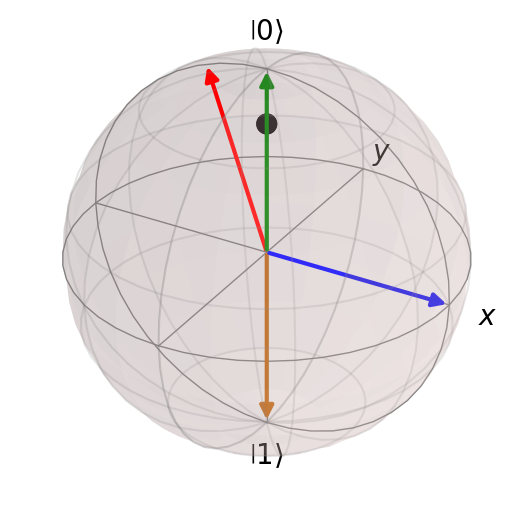
\includegraphics[width=0.5\textwidth]{bloch_sphere.png}
      \captionof{figure}{Bloch sphere indicating the different decompositions. The black circle indicates the position of $\rho$. The states in green and yellow are the states $\ket{0}$ and $\ket{1}$ respectively. The states in blue and red are the states $\ket{+}$ and $\ket{\psi}$ respectively. The lines connecting each of these pairs of states passes through $\rho$.}\label{fig:bloch}
    \end{minipage}}
  \end{proof}
\end{solution}
